\documentclass[aspectratio=169]{beamer}
\usepackage[utf8]{inputenc}
\usepackage[T1]{fontenc}
\usepackage[french]{babel}
\usepackage{graphicx}
\usepackage{pgfpages}

\graphicspath{{images/}}

% Theme simple et elegant
\usetheme{Boadilla}
\usecolortheme{seahorse}

% Activer les notes pour le presentateur (commentez pour un PDF simple)
% \setbeameroption{show notes on second screen=right}

\title{Logique et Fondements de l'Informatique}
\subtitle{L'ère des Assistants de Preuve}
\author{Introduction}
\date{Leçon 1}

\begin{document}

% SLIDE 1
\begin{frame}
  \titlepage
  \note{
    Bonjour à tous et bienvenue dans la seconde partie de ce cours. \\
    Aujourd'hui, nous allons passer de la théorie pure (le papier) à la pratique mécanique.\\
    Question d'introduction : Comment sait-on qu'une démonstration est juste ? L'humain est faillible, le langage naturel est ambigu. On va utiliser une machine comme arbitre absolu.
  }
\end{frame}

% SLIDE 2
\begin{frame}{Qu'est-ce qu'un Assistant de Preuve ?}
  \begin{itemize}
    \item L'humain fournit les idées (spécification, argumentation).
    \item La machine vérifie rigoureusement chaque étape de déduction.
    \item Aucun saut logique n'est toléré.
  \end{itemize}
  % Remplacer example-image par le logo de Rocq ou une capture d'ecran
  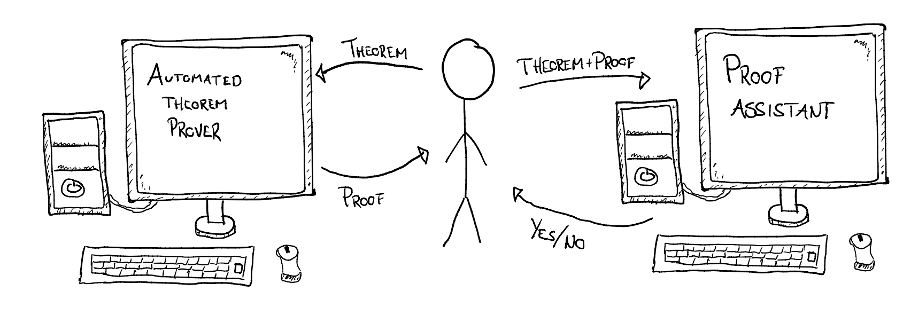
\includegraphics[width=\textwidth]{proofassistant.png}
  \note{
    Bien faire la distinction avec un "démonstrateur automatique" (qui cherche la solution tout seul). Ici, c'est une collaboration. Le système vérifie un arbre de preuve formel avec un tout petit noyau de confiance.
  }
\end{frame}

% SLIDE 3
\begin{frame}{Une brève histoire de la mécanisation}
  \begin{itemize}
    \item \textbf{1968 - Automath :} N.G. de Bruijn aux Pays-Bas. Première tentative de vérifier des mathématiques par ordinateur.
    \item \textbf{1972 - LCF :} Robin Milner invente le concept de "Tactiques" pour faciliter la construction à la fois automatique et interactive des preuves.
    \item \textbf{1984 - Calcul des Constructions :} Thierry Coquand et Gérard Huet (Inria).
    \item \textbf{1989 - Coq (aujourd'hui Rocq) :} Naissance du système que nous allons utiliser.
    \item \textbf{Aujourd'hui :} Rocq, Lean, Agda, Isabelle/HOL {\small(et d'autres moins connus/plus spécialisés).}
  \end{itemize}
  \note{
    Mentionner que la France (Inria) a joué un rôle historique massif dans ce domaine. Le projet Automath de De Bruijn a donné le "critère de de Bruijn" (avoir un noyau de vérification minimaliste).
  }
\end{frame}

% SLIDE 4
\begin{frame}{Le pont théorique : Curry-Howard}
  \begin{center}
    \LARGE \textbf{Propositions = Types}\\
    \LARGE \textbf{Preuves = Programmes}
  \end{center}
  \vspace{0.5cm}
  \begin{itemize}
    \item \textbf{Théorie de la démonstration} $\longleftrightarrow$ \textbf{Théorie des types}
    \item Prouver un théorème, c'est écrire un programme (un $\lambda$-terme) qui "compile" avec le type de ce théorème.
  \end{itemize}
  \note{
    Rappeler ce qu'ils ont vu lors des 6 premières semaines de cours. C'est la justification épistémologique de l'outil : on ne fait pas "confiance" à l'ordinateur à l'aveugle, on lui demande de vérifier le typage d'un lambda-terme pur.
  }
\end{frame}

% SLIDE 5
\begin{frame}{Un raz-de-marée en Mathématiques}
  \begin{itemize}
    \item \textbf{Vérification de l'état de l'art :}
      \begin{itemize}
        \item \textbf{2005 - Théorème des Quatre Couleurs :} Preuve formelle en Rocq par Georges Gonthier~\cite{gonthier2008fourcolor}.
        \item \textbf{2014 - Conjecture de Kepler :} Projet Flyspeck (Isabelle/HOL Light) par Thomas Hales~\cite{hales2017flyspeck}.
        \item \textbf{2021 - Liquid Tensor Experiment :} Peter Scholze (Médaille Fields) fait vérifier son propre théorème par la communauté Lean~\cite{scholze2021liquid}.
      \end{itemize}
    \item \textbf{Machine Learning \& IA :}
      \begin{itemize}
        \item \textbf{2024 - AlphaProof :} Médaille d'argent (avec AlphaProof) aux Olympiades Internationales de Mathématiques~\cite{alphaproof2024}.
        \item \textbf{2026 - Mathlib \& Conjectures d'Erdős :} Résolution automatisée de problèmes ouverts via Lean par des startups et des mathématiciens~\cite{erdosproblems}.
      \end{itemize}
  \end{itemize}
  \note{
    Insister sur le fait que ce n'est plus un jouet pour informaticiens. Les meilleurs mathématiciens du monde commencent à douter de la capacité de la relecture par les pairs face à la complexité des mathématiques modernes, et se tournent vers les assistants de preuve. Mentions de Hoskinson ou des grands modèles de langages (LLM) qui traduisent la pensée informelle en Lean/Rocq.
  }
\end{frame}

% SLIDE 6
\begin{frame}{Industrie et Méthodes Formelles}
  \begin{columns}
    \begin{column}{0.6\textwidth}
      Comment s'assurer qu'un système critique (avion, métro, nucléaire) n'a \textbf{aucun} bug ? Les tests ne suffisent pas.
      \vspace{0.3cm}
      \begin{itemize}
        \item \textbf{CompCert~\cite{leroy2009compcert} :} Compilateur C certifié en Rocq (0 bug de compilation mathématiquement garanti).
        \item \textbf{seL4~\cite{klein2009sel4} :} Noyau de système d'exploitation sécurisé et prouvé formellement dans Isabelle.
        \item \textbf{Ligne 14 du Métro Parisien~\cite{behm1999meteor} :} Développement des pilotes automatiques (projet METEOR) avec 0 bug détecté à l'aide de la Méthode B.
        \item \textbf{Signal \& Protocole MLS~\cite{wallez2025mls} :} Le protocole de messagerie de groupe utilisé par Signal a été certifié par preuves formelles automatisées.
      \end{itemize}
    \end{column}
    \begin{column}{0.4\textwidth}
      % Remplacer par une image d'un avion ou de code C
      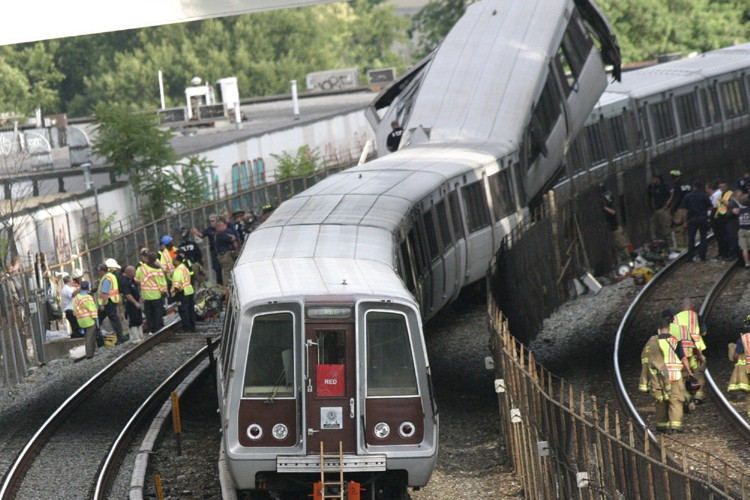
\includegraphics[width=\textwidth]{88995-accident-produit-17h00-proche-limite.jpg}
    \end{column}
  \end{columns}
  \note{
    Faire le lien avec le titre du cours "Fondements de l'informatique". La logique permet des garanties de sécurité qui sont impossibles avec les méthodes d'ingénierie logicielle classiques.
  }
\end{frame}

% SLIDE 7
\begin{frame}{Applications en philosophie analytique}
  La formalisation permet de débusquer les prémisses cachées, les contradictions, et de désambiguïser les concepts :
  \begin{itemize}
    \item \textbf{Métaphysique :} Formalisation par Zalta des "objets abstraits" via la logique computationnelle dans Isabelle/HOL~\cite{kirchner2017zalta}.
    \item \textbf{Théologie :} Vérification formelle par ordinateur des arguments ontologiques (Anselme, variante modale de Gödel)~\cite{benzmuller2013goedel}.
    \item \textbf{Éthique classique :} Tentatives de mécanisation de l'\emph{Éthique} de Spinoza (écrite initialement \emph{more geometrico}) en Coq~\cite{pommeret2025spinoza}.
  \end{itemize}
  \note{
    C'est pour les motiver ! Le but est de leur montrer que l'outil est applicable à leur discipline. L'ordinateur met en évidence les axiomes implicites utilisés par les philosophes du passé.
  }
\end{frame}

% SLIDE 8
\begin{frame}{Plan du Cours (6 semaines)}
  \begin{itemize}
    \item \textbf{Semaine 1 :} Du $\lambda$-calcul à Rocq
    \item \textbf{Semaine 2 :} Logique propositionnelle, intuitionniste, classique
    \item \textbf{Semaine 3 :} Épistémologie des types de données
    \item \textbf{Semaine 4 :} Logique des prédicats et égalité
    \item \textbf{Semaine 5 :} Programmation fonctionnelle et types inductifs
    \item \textbf{Semaine 6 :} Vérification de programmes et fiabilité de l'IA
  \end{itemize}
  \note{
    Présentation rapide du programme des 6 prochaines semaines pour donner une vue d'ensemble du module.
  }
\end{frame}

% SLIDE 9
\begin{frame}{Au menu aujourd'hui : Anatomie de Rocq}
  Rocq est composé de \textbf{3 niveaux de langage} :
  \vspace{0.3cm}
  \begin{enumerate}
    \item \textbf{Le Vernaculaire} : Les commandes pour "parler" au système (\texttt{Section}, \texttt{Definition}, \texttt{Lemma}).
    \item \textbf{Gallina} : Le langage fonctionnel pur ($\lambda$-calcul) où vivent les termes et les types. L'artefact final de vérité.
    \item \textbf{Ltac} : Le langage de "Tactiques" (\texttt{intros}, \texttt{apply}). Un méta-langage interactif pour aider l'humain à construire le terme Gallina étape par étape.
  \end{enumerate}
  \note{
    Annoncer la transition vers le TP : "Nous allons maintenant ouvrir nos navigateurs et voir ces 3 langages en action avec jsCoq."
  }
\end{frame}

% SLIDE 10
\begin{frame}[allowframebreaks]{Bibliographie}
  \begin{thebibliography}{9}
    \setbeamertemplate{bibliography item}[text]

    \bibitem{leroy2009compcert}
    Xavier Leroy.
    \newblock \emph{Formal verification of a realistic compiler}.
    \newblock Communications of the ACM, 2009.
    \newblock \url{https://dl.acm.org/doi/10.1145/1538788.1538814}

    \bibitem{klein2009sel4}
    Gerwin Klein et al.
    \newblock \emph{seL4: Formal verification of an OS kernel}.
    \newblock SOSP, 2009.
    \newblock \url{https://dl.acm.org/doi/10.1145/1629575.1629596}

    \bibitem{behm1999meteor}
    P. Behm, P. Benoit, A. Faivre, and J.-M. Meynadier.
    \newblock \emph{Météor: A successful application of B in a large project}.
    \newblock FM'99—Formal Methods, 1999.
    \newblock \url{https://link.springer.com/chapter/10.1007/3-540-48119-2_22}

    \bibitem{wallez2025mls}
    Théophile Wallez.
    \newblock \emph{Cadriciel de vérification pour la messagerie de groupe sécurisée}.
    \newblock Thèse de doctorat, Inria Paris, 2025.
    \newblock \url{https://theses.fr/s275565}

    \bibitem{gonthier2008fourcolor}
    Georges Gonthier.
    \newblock \emph{Formal Proof—The Four Color Theorem}.
    \newblock Notices of the AMS, 2008.
    \newblock \url{https://www.ams.org/notices/200811/tx081101382p.pdf}

    \bibitem{hales2017flyspeck}
    Thomas Hales et al.
    \newblock \emph{A Formal Proof of the Kepler Conjecture}.
    \newblock Forum of Mathematics, Pi, 2017.
    \newblock \url{https://doi.org/10.1017/fmp.2017.1}

    \bibitem{scholze2021liquid}
    Peter Scholze et al.
    \newblock \emph{Liquid Tensor Experiment}.
    \newblock 2021.
    \newblock \url{https://leanprover-community.github.io/liquid/}
    \newblock \url{https://pat2023.icube.unistra.fr/slides/slides-pat2023-commelin-talk2.pdf}

    \bibitem{alphaproof2024}
    Google DeepMind.
    \newblock \emph{AlphaProof and AlphaGeometry 2 solve IMO problems}.
    \newblock 2024.
    \newblock \url{https://deepmind.google/discover/blog/ai-solves-imo-problems-at-silver-medal-level/}

    \bibitem{erdosproblems}
    natsothanaphan.
    \newblock \emph{AI contributions to Erdős problems}.
    \newblock 2026.
    \newblock \url{https://github.com/teorth/erdosproblems/wiki/AI-contributions-to-Erd\%C5\%91s-problems/}

    \bibitem{kirchner2017zalta}
    Daniel Kirchner.
    \newblock \emph{Representation and Partial Automation of the Principia Logico-Metaphysica in Isabelle/HOL}.
    \newblock Archive of Formal Proofs, 2017.
    \newblock \url{https://www.isa-afp.org/entries/PLM.html}

    \bibitem{benzmuller2013goedel}
    Christoph Benzmüller and Bruno Woltzenlogel Paleo.
    \newblock \emph{Formalization, Mechanization and Automation of Gödel's Proof of God's Existence}.
    \newblock arXiv preprint, 2013.
    \newblock \url{https://arxiv.org/abs/1308.4526}

    \bibitem{pommeret2025spinoza}
    Luc Pommeret.
    \newblock \emph{Preuves en déduction naturelle du livre I de l'Éthique de Spinoza}.
    \newblock Document de travail (lucpommeret.com), 2025.
    \newblock \url{https://lucpommeret.com/assets/De_Deo.pdf}

  \end{thebibliography}
\end{frame}

\end{document}